\section{Phase 1: Online Survey}
\subsection{Methodology}
We conducted a preliminary survey to identify important aspects of customers' in-store and online shopping experiences. We asked participants to identify the three most important pieces of information involved their shopping decisions, what they did and did not like about existing in-store and online shopping experiences, and ways they currently use technology in shopping. \todo{does this feel like a reasonable synopsis?}  \todo{JRB: Yes, except I would like to know if these were open-ended questions or not.}
We used the responses from our online survey to isolate factors of in-store and online shopping that were most important to our participants.  The survey consisted of both qualitative and quantitative questions.  We aggregated qualitative responses to open-ended questions and found broad themes.  \todo{Can you add some details about how you analyzed this data here?}  \todo{JRB: Amen! Ethan and Matt, talk about this one? Was it a thematic analysis? Did you just see what people were saying? If you can describe what you did to me in casual english, I can help you science it up.} \todo{MW: Okay, help me science it.}


\subsection{Findings}
\begin{figure}
	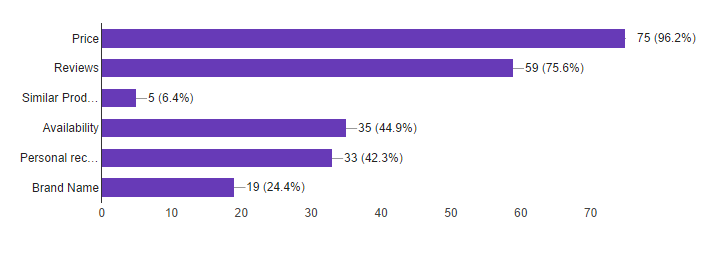
\includegraphics[width=0.9\columnwidth]{figures/ShoppingFactors}
	\caption{Most important factors in making shopping decisions}
	\label{figures:ShoppingFactors}
\end{figure}

We collected responses from 78 participants over social media.  We found that participants appreciate the immediacy and physical interaction with products in a store.  Cited drawbacks of shopping in-store were a lack of ability to comparison shop, inability to get the lowest price and/or feeling that they are paying too much, and store staff trying to influence purchase decisions.  Participants said they appreciate the freedom from store location and hours, \todo{I'm not sure what "freedom from store location and hours" means - EH} and time-to-completion of online shopping, \todo{I'm confused as to whether you're talking about things participants appreciate about in-store shopping or about online shopping} but said they dislike the shipping charges and wait times associate with online shopping.  Figure \ref{figures:ShoppingFactors} details participants' responses when prompted for their three most important factors in making shopping decisions.  We also found that users are willing to spend more time researching more expensive products.